\clearpage
\subsection{Tiles}
\subsubsection{Idea}
A very obvious feature that can be retrieved from an image is tiles, more specifically how many tiles it contains. This section will explain how a tile can be recognised and how these tiles are used to differentiate between different regions of the path. 
\subsubsection{Recognising tiles}
Shadows, lack of light, dirt  and blurry images are real culprits when it comes down to recognising tiles. To get the best results, the search for rectangles is repeated during multiple iterations. Each iteration applies a different filter to counteract the shadows, dirt and bad image quality. The lack of light is dealt with by repeating the search twice, once on the normal image and once on the image with increased contrast. This repitition is necessary because increasing the contrast on an already bright image reduces the amount of tiles that are be found. The results of the normal and manipulated image are added up and considered the global result for the given image. 
\npar
The search iterations  consist of a few filters that counteract shadows, dirt and bad image quality. Each set of iterations initially converts the received image to a grayscale image. The first iteration applies a Canny\footnote{\url{http://docs.opencv.org/modules/imgproc/doc/feature_detection.html?highlight=canny\#canny}} filter, which is used for finding edges in an image. The aforementioned culprits cause the Canny edges to leave gaps where there shouldn't be. Dilating\footnote{\url{http://docs.opencv.org/modules/imgproc/doc/filtering.html?highlight=dilate\#void dilate(InputArray src, OutputArray dst, InputArray kernel, Point anchor, int iterations, int borderType, const Scalar& borderValue)}} the result from Canny fills up most of these gaps. The Canny and dilate results are shown the figures below.  

\begin{figure}[ht]
\centering
\begin{subfigure}{.5\textwidth}
  \centering
  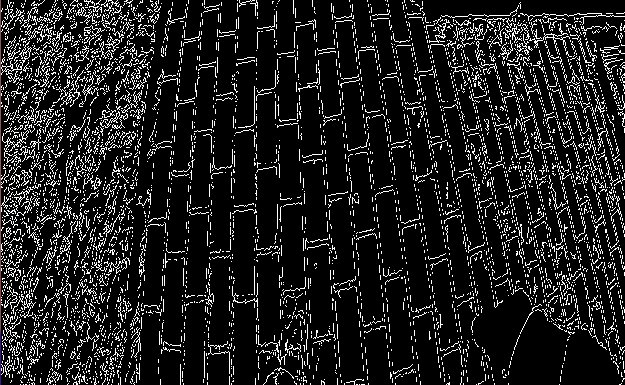
\includegraphics[width=.9\textwidth]{canny}
  \caption{Canny filter\label{canny}}
\end{subfigure}%
\begin{subfigure}{.5\textwidth}
  \centering
  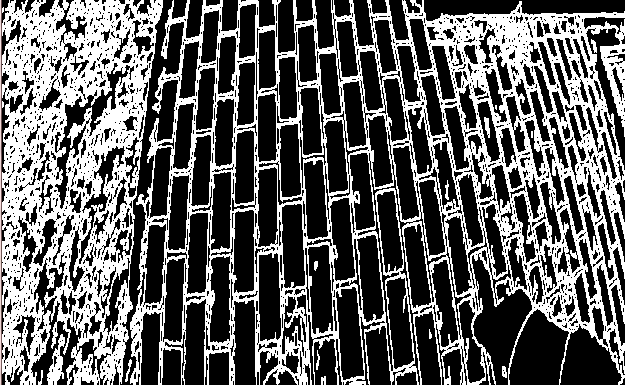
\includegraphics[width=.9\textwidth]{dilate}
  \caption{Dilate\label{dilate}}
\end{subfigure}
\caption{Canny and dilate\label{canny_dilate}}
\end{figure}

The result after dilate appears near perfect, which begs the question why any other filter is required. The answer is simple: Canny reacts very poorly to dirt. As an example consider the left side of the images. This side consists of grass, which is recognised by Canny is a spaghetti of edges. If there was a tile in there, it would be heavily distorted by this grass. The same applies to dirt on a tile. The reason why Canny is used, is because it is not affected by tiles with a gradient shading, which is the downfall of the second filter.
\npar
The remaining iterations apply the same type of filter with a different threshold on each iteration. The pixels of the initial grayscale image with a whiteness intensity above the threshold are copied into a new image. Because tiles are separated by dark grooves, this new image will only contain the tiles. Or rather, this is the goal. Multiple thresholds are required to deal with more or less sunlight making the tiles brighter or darker. Similar to the Canny result, the lines contouring the tiles may not appropriately connect. Erode\footnote{\url{http://docs.opencv.org/modules/imgproc/doc/filtering.html?highlight=dilate\#erode}} is used to shrink the tiles a little bit, improving the boundaries around those tiles. The result is shown below.

\begin{figure}[ht]
\centering
\begin{subfigure}{.5\textwidth}
  \centering
  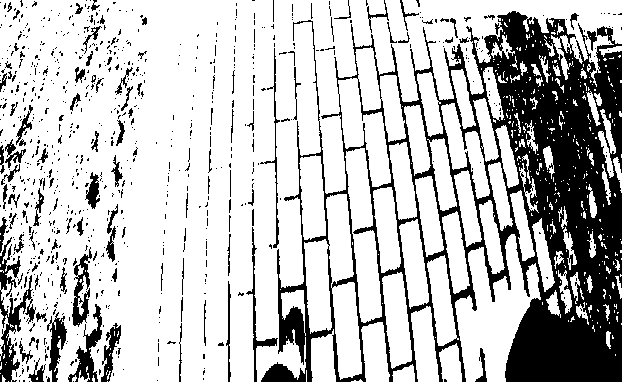
\includegraphics[width=.9\textwidth]{gray}
  \caption{Color intensity thresholding\label{gray}}
\end{subfigure}%
\begin{subfigure}{.5\textwidth}
  \centering
  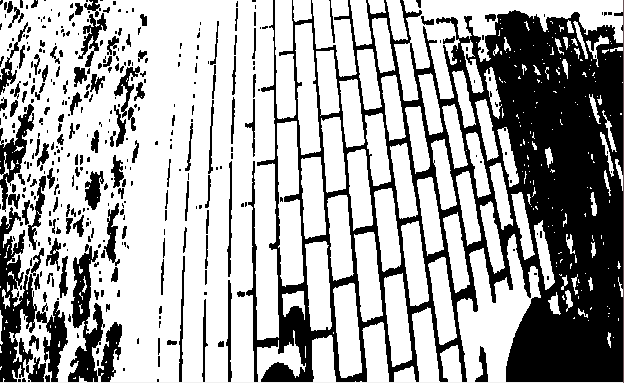
\includegraphics[width=.9\textwidth]{erode}
  \caption{Erode\label{erode}}
\end{subfigure}
\caption{Thresholding and erode\label{gray_erode}}
\end{figure}

\npar
Each filter results in a bunch of contours around the existing tiles. These contours can be retreived with the findContours\footnote{\url{http://docs.opencv.org/modules/imgproc/doc/structural_analysis_and_shape_descriptors.html?highlight=findcontours\#findcontours}} function. This will return every contour found in the image, not just the ones belonging to the tiles. Extracting the useful contours is done in three steps:
\begin{enumerate}
\item{approxPolyDP\footnote{\url{http://docs.opencv.org/modules/imgproc/doc/structural_analysis_and_shape_descriptors.html\#approxpolydp}} is used to approximate the contours with a polygonal.}
\item{Tile contours should have 4 vertices, so every approximated contour that doesn't match this constraint is dropped.}
\item{A tile is a rectangle, meaning its corners should be at a 90 degree angle. Calculating this angle happens through simple math, using the following formula: $v \cdot w = ||v|| * ||w|| cos q$. Every contour that has corners with a cosine greater than $0.3$ is dropped. Note that $0.3$ is chosen as a margin of error, allowing slightly less than perfect rectangles to be accepted. }
\end{enumerate}

\subsubsection{Using tile sizes}
Finding tiles as described above, yields every rectangle ranging from only a few pixels to a square the size of the frame itself. The next step is filtering out unwanted sizes and grouping them into sizes that match certain real tile sizes. The size groups are chosen as following:
\begin{enumerate}
\item{Small tiles: 801 to 4500 pixels}
\item{Medium tiles: 4501 to 19000 pixels}
\item{Large tiles: 19000 to 100000 pixels}
\end{enumerate}
Finding these sizes has been done through trail and error. They have proven to be the best boundaries between the tile sizes found in the given video fragments.
\subsubsection{Setting the boundaries of regions}
Initially, finding proper boundaries for certain regions based on tile sizes proved to be problematic. A tile further ahead appears smaller than it really is, clouding the results with wrong tile sizes. One option could be to manipulate the perspective, turning the image in a top down view. This method however is rather difficult and could potentially distort the boundaries of certain tiles even more. A second approach was used: only use the bottom half of the image.  This approach is quite logical, only take the tiles into account that the person is on right now. Tiles in the distant can be quite irrelivant and can, due to minor detours, have nothing to do with the actual route. The result for first video fragment, the path from the university campus to the train station, is shown in Figure \ref{grafiek_tegelgroottes}.

\begin{figure}[ht]
\centering
  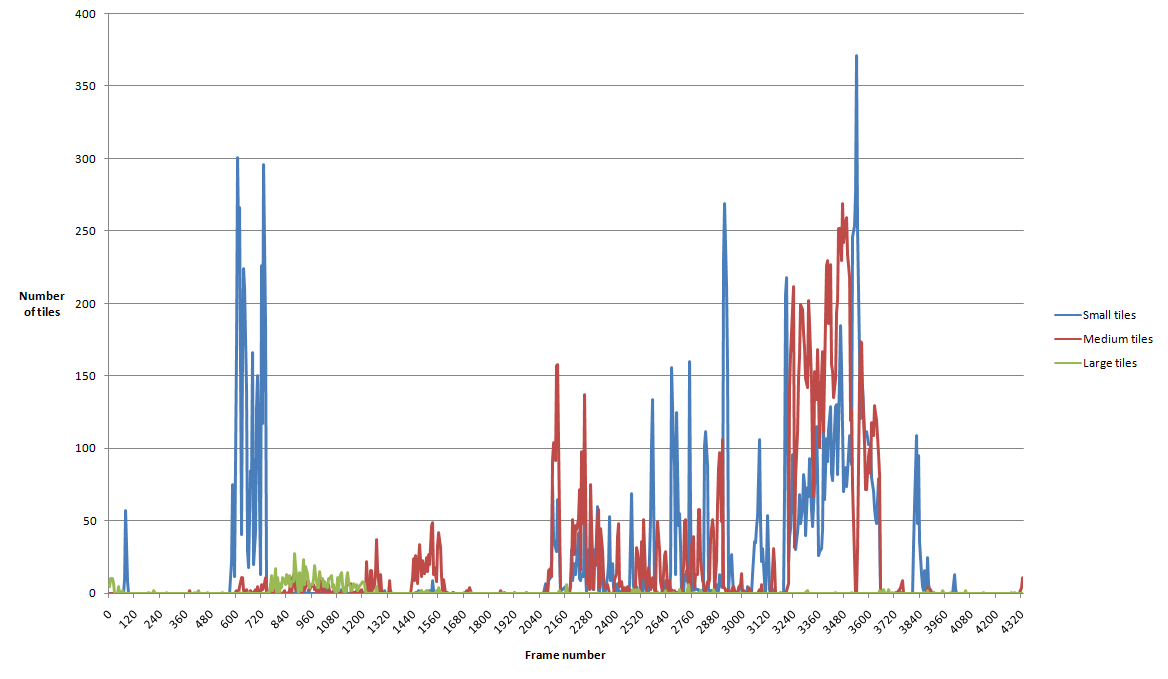
\includegraphics[width=1.1\textwidth]{grafiek_tegelgroottes}
  \caption{Tile count for the first video fragment\label{grafiek_tegelgroottes}}
\end{figure}
The first half of the graph above marks very distinct regions based on the absence or presence of certain tile sizes. The second half is not as fortunate. The Sint-Denijslaan consists of frequent alterations between small and medium tiles, making it difficult to mark large enough regions with a common tile size. Near the end the medium tiles see a significant increase in number. Unfortunately this cannot be used to mark a new region, because there are too many factors that can influence the number of tiles recognised. The result would be too unreliable, especially considering this region lies immediately next to its counterpart with lower, but still significant numbers. For this reason, the boundary leading up to its neighbouring region would have to be be very clear.  

\subsubsection{Conclusion}
Using tile sizes as a feature is definitly an option. It is perfectly suited for giving a raw estimation of where the user is located. This estimation can then be refined by using additional features.
\clearpage
